\documentclass[a4paper]{article}
\usepackage{amsmath}
\usepackage{amsfonts}
\usepackage{amssymb}
\usepackage{ucs}
\usepackage[T2A]{fontenc}
\usepackage[utf8]{inputenc}
\usepackage[english,bulgarian]{babel}
\usepackage{graphicx}
\usepackage{url}
\usepackage{textcomp}
\usepackage{tabularx}
\usepackage{array}
\usepackage[margin=1.5in]{geometry}
\usepackage[unicode]{hyperref}
\usepackage{listings}
\usepackage{color}
\definecolor{gray}{rgb}{0.6,0.6,0.6}
\usepackage[usenames,dvipsnames]{xcolor}
\lstset{language=C++,captionpos=b,
tabsize=4,frame=lines,
basicstyle=\script\ttfamily,
keywordstyle=\color{blue},
commentstyle=\color{gray},
stringstyle=\color{violet},
breaklines=true,showstringspaces=false}


\usepackage{fancyhdr}
\setlength{\headheight}{15pt}
 
\pagestyle{fancyplain}


\addto\captionsbulgarian{%
  \renewcommand{\contentsname}%
    {Содржина}%
  \renewcommand{\tablename}%
    {Табела}%
  \renewcommand{\figurename}%
    {Слика}%
  \renewcommand{\bibname}%
    {Библиографија}%
  \renewcommand{\listfigurename}%
    {Листа на слики}%
  \renewcommand{\listtablename}%
    {Листа на табели}%
}

\rhead{\textsc{Софтверско инженерство}}

\lhead{Аудиториски вежби 3}
\lfoot{}
\cfoot{\thepage}
\rfoot{}
\usepackage{fancyvrb}
\usepackage{xcolor}
\usepackage{textcomp}

\begin{document}

\section{STL компоненти}

\subsection{Вовед}

STL содржи шест главни видови на компоненти:

\begin{itemize}
  \item containers
  \item generic algorithms
  \item iterators
  \item function objects
  \item adaptors
  \item allocators
\end{itemize}

Во STL контејнерите се објекти кои се користат за чувување на колекци и од други
објекти. 
Постојат две категории на STL контејнери: 
\begin{itemize}
  \item секвенцијални контејнери
  \item сортирани асоцијативни контејнери. 
\end{itemize}

\begin{figure}[htb]
\centering
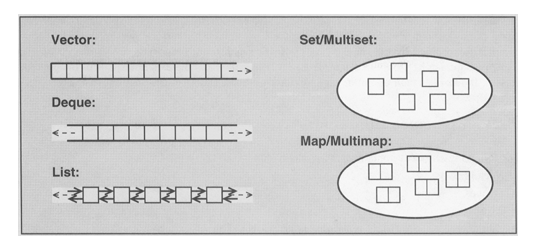
\includegraphics[scale=.5]{images/container_types}
\caption{Видови на контејнери}
\label{fig:container_types}
\end{figure}

\subsection{Секвенцијални контејнери}

Секвенцјалните контејнери организираат колекција од објекти, сите од ист тип T,
во строго линеарен режим. Во оваа група на контејнери спаѓаат: 

\begin{itemize}
  \item \texttt{vector<T>} - Обезбедува случаен пристап на секвенца со променлива
  должина. Случаен пристап означува дека времето за да се дојде до i-от елемент 
  од секвенцата е константно, односно не зависи од i и со константно време
  потребно за вметнување и бришење на елементи од крајот. Дефинирани се со
  користење на полиња.
  \item \texttt{deque<T>} - Обезбедува случаен пристап на секвенца со променлива должина,
  со константно време за вметнување и бришење на елементи од почетокот и крајот.
  Дефинирани се со користење на полиња со две нивоа.
  \item \texttt{list<T>} - Обезбедува линеарен пристап на секвененца со
  променлива. должина(O(N), каде N е моменталната должина), но со константно време потребно за вметнување и
бришење на било која позиција во секвенцата. Дефинирани се со користење на двојно
поврзани листи.
\end{itemize}

\subsection{Асоцијативни контејнери}

Во групата на сортирани асоцијативни контејнери спаѓаат контејнери со способност за
враќање на објекти базирани на клучеви. Елементите се сортирани па со примена на
бинарно пребарување многу брзо може да се пронајде даден елемент. Во STL постојат
четири типови на сортирани асоцијативни контејнери:
\begin{itemize}
  \item \texttt{set<Key>}
  \item \texttt{multiset<Key>}
  \item \texttt{map<Key,T>}
  \item \texttt{multimap<Key,T>}    
\end{itemize}

\subsection{Заеднички операции за сите контејнери}

Секоја класа која репрезентира одреден контејнер обезбедува \texttt{default}
конструктор, copy конструктор и деструктор. Исто така постои можност за
иницијализација на контејнер со елементи од даден опсег, овој конструктор е
понуден за да се овозможи иницијализација на контејнер со елементи од друг
контејнер, поле или пак преку стандарден влез. Сите овие конструктори се
функциски темплејти па соодветно се разликуваат и типовите на елементи за кои се
однесуваат.

\begin{center}
  \begin{tabular}{ | l | p{7cm} |}
    \hline
    \texttt{ContType c} & Креира празен контејнер без елементи \\
    \hline
    \texttt{ContType c1(c2)} & Копира контејнер од истиот вид  \\
    \hline
    \texttt{ContType c(beg,end)} & Креира контејнер и го инцијализира со копија
    на елементите од [beg,end) \\
    \hline
    \texttt{c.~ContType()} & Ги брише сите елементи и ја ослободува меморијата  \\
    \hline
    \texttt{c.size()} & Го враќа бројот на елементи \\
    \hline
    \texttt{c.empty()} & Враќа дали контејнерот е празен (исто со \texttt{size()==0},
    но може да биде побрзо) \\
    \hline
    \texttt{c.max\_size()} & Го враќа максималниот можен број на елементи
    \\
    \hline
    \texttt{c1 == 2} & Враќа дали \texttt{c1} е еднаков на \texttt{c2} \\
    \hline
    \texttt{c1 != c2} & Враќа дали \texttt{c1} не е еднаков на \texttt{c2}
    (исто со \texttt{!(c1==c2)})
    \\
    \hline
    \texttt{c1 < c2} & Враќа дали \texttt{c1} е помал од \texttt{c2} \\
    \hline
    \texttt{c1 > c2} & Враќа дали \texttt{c1} е поголем од \texttt{c2}
    (исто со \texttt{c2 < c1}) \\
    \hline
    \texttt{c1 <= c2} & Враќа дали \texttt{c1} е помало или еднакво на
    \texttt{c2} (исто со \texttt{!(c2 < c1)}) \\
    \hline 
    \texttt{c1 >= c2} & Враќа дали \texttt{c1} е поголемо или еднакво на
    \texttt{c2} (исто со \texttt{!(c1 < c2)}) \\
    \hline
    \texttt{c1 = c2} & Ги доделува сите елементи од \texttt{c1} на \texttt{c2}
    \\
    \hline
    \texttt{c1.swap(c2)} & Ги менува податоците од \texttt{c1} и \texttt{c2} \\
    \hline
    \texttt{swap(c1,c2)} & Исто (како глобална функција)
    \\
    \hline
    \texttt{c.begin()} & Враќа итератор од првиот елемент
    \\
    \hline
    \texttt{c.end()} & Враќа итератор од позицијата после последниот елемент\\
    \hline
    \texttt{c.rbegin()} & Враќа превртен итератор од првиот елемент за
    обратна итерација
    \\
    \hline
    \texttt{c.rend()} & Враќа превртен итератор од позицијата после
    последниот елемент за обратна итерација\\
    \hline
    \texttt{c.insert(pos,elem)} & Вметнува копија од \texttt{elem} на позиција
    \texttt{pos}
    \\
    \hline
    \texttt{c.erase(beg,end)} & ги отстранува сите елементи во опсегот [beg,end)\\
    \hline
    \texttt{c.clear()} & ги отстранува сите елементи-празен контејнер \\
    \hline
    \texttt{c.get\_allocator()} & го враќа меморискиот модел за контејнерот \\
    \hline
  \end{tabular}
\end{center}

\textsc{Пример 1}

\begin{lstlisting}
list<int> l;
vector<float> c(l.begin(),l.end());
int array[] = { 2, 3, 17, 33, 45, 77 };
set<int> c(array, array + sizeof(array) / sizeof(array[0]));
deque<int> d(istream_iterator<int>(cin), istream_iterator<int>());
\end{lstlisting}

Операциите за споредба се потчинуваат на следниве правила:

\begin{enumerate}
  \item Двата контејнери мора да содржат ист тип
  \item Два контејнери се еднакви ако нивните елементи се еднакви и ако се во ист
редослед
  \item При користење на операциите (<,> ...) се користи лексикографска
  споредба.
\end{enumerate}
За споредба на контејнери со различни типови мора да се користат генеричките
алгоритми за споредба.

\section{Вектори}
Векторот всушност претставува динамичко поле. Ако користиме \texttt{vector},
мора да ја вклучиме дататоката заглавје \texttt{<vector>}:
\begin{verbatim}
#include <vector>
\end{verbatim}
Векторот е дефиниран како темплејт класа во рамките на \texttt{std}:

\begin{lstlisting}
namespace std {
	template <class T,
	class Allocator = allocator<T> >
	class vector;
}
\end{lstlisting}

Елементите на векторот можат да бидат од било кој тип \texttt{T}. Вториот
аргумент го дефинира меморискиот модел (\texttt{default} мемориски модел е
\texttt{allocator}, кој е обезбеден во C++ standard library). Векторите
овозможуваат случаен пристап, односно може да се пристапи до било кој елемент
директно за константно време. Векторите се оптимизирани за додавање и бришење на
елементи на крајот. Ако вметнуваме или бришеме елементи во средината или на
почетокот перформансите значително се намалуваат, поради фактот што секој
елемент кој следи после елементот кој се додава мора да се помести на друга
позиција (се повикува операторот за доделување). Дополнителен оператор за
манипулација со големината на векторот е \texttt{capacity()} функцијата која го
враќа бројот на објекти кои може да ги содржи векторот во неговата вистинска
меморија. Ако се надмине \texttt{capacity()}, векторот мора да изврши релокација
на неговата внатрешна меморија. За да се избегне релокацијата на меморија, може
да се користи \texttt{reserve()} за да обезбедиме одреден капацитет. 

\textsc{Пример 2:}
\begin{lstlisting}
vector<int> v;
v.reserve (80);
vector<T> v(5); //povik na default constructor
\end{lstlisting}

Во следнава табела се дадени сите конструктори и деструктори за вектор класата.
\begin{figure}[htb]
\centering
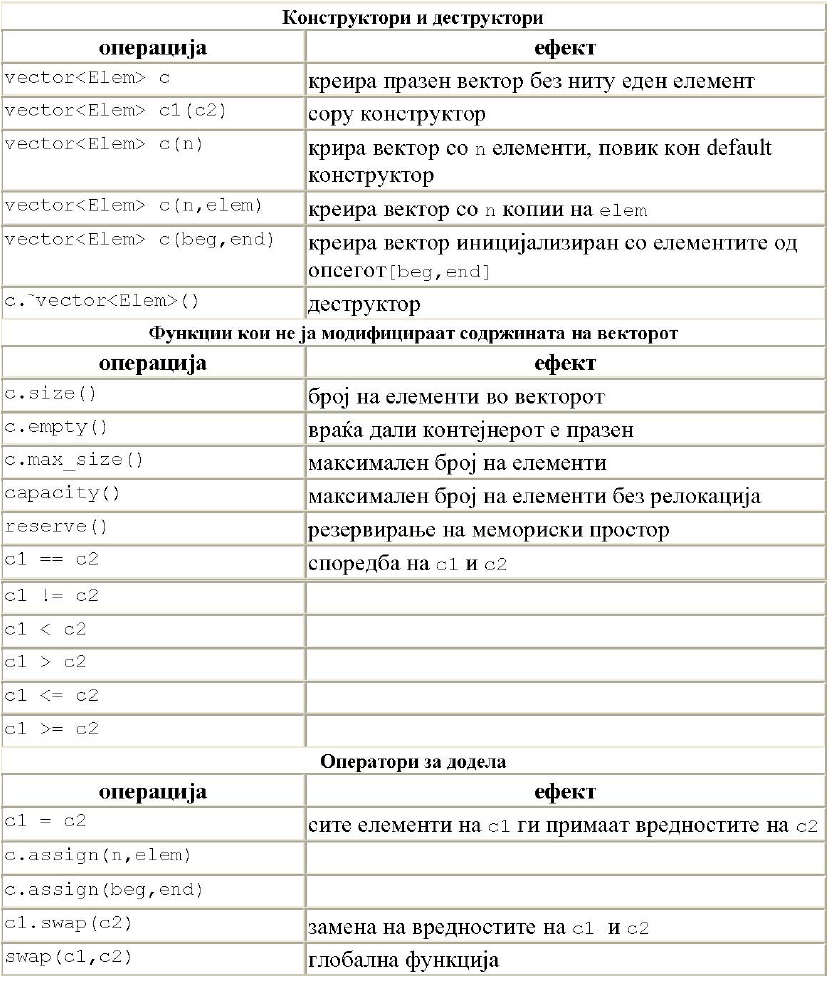
\includegraphics[width=\textwidth]{images/vector}
\caption{Конструктори и методи на вектор}
\label{fig:vector}
\end{figure}

Во следната табела се дадени операциите за директен пристап до елементите кои се
наоѓаат во векторот (првиот елемент има индекс 0 додека последниот елемент има
индекс \texttt{size() - 1}). За неконстантни вектори овие операции враќаат
референца кон елементот.


\begin{figure}[htb]
\centering
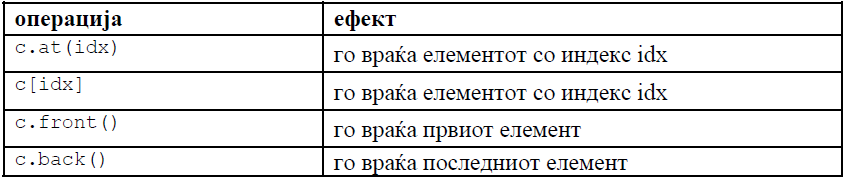
\includegraphics[width=\textwidth]{images/operations}
\label{fig:vector_operations}
\end{figure}

Само кај операторот \texttt{at()} се врши проверка на опсегот на индексот
(\texttt{out\_of\_range exception}). Сите останати функции не вршат проверка на
опсегот.

\begin{figure}[htb]
\centering
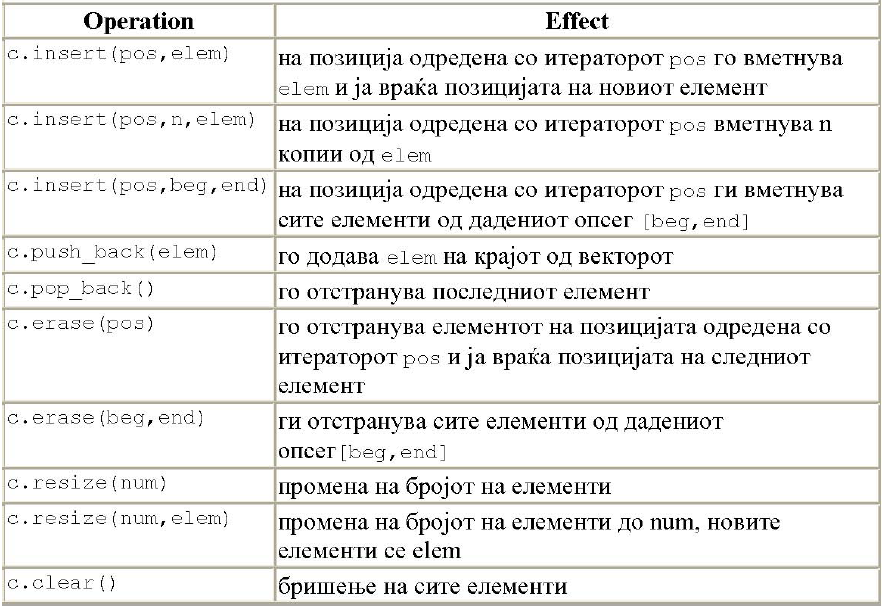
\includegraphics[width=\textwidth]{images/add_remove}
\caption{Додавање и бришење елементи}
\label{fig:add_remove}
\end{figure}
   
\textsc{Пример 3}

\begin{lstlisting}
vector<Elem> coll;
coll[5] = elem;
cout << coll.front ();
vector<Elem> coll;
if (coll.size() > 5) {
	coll [5] = elem;
}
if (!coll.empty()) {
	cout << coll.front();
}
coll.at(5) = elem;
\end{lstlisting}  

Вектор класата обезбедува оператори кои враќаат итератори (станува збор за
итератори со случаен пристап). 
   
\begin{center}
  \begin{tabular}{ | l | p{7cm} |}
	\hline
	\textbf{операција} & \textbf{ефект}\\
	\hline
	\texttt{c.begin()} & враќа итератор со случаен пристап за првиот елемент \\
	\hline
	\texttt{c.end()} &  враќа итератор со случаен пристап за елментот после
	последниот\\ 
	\hline
	\texttt{c.rbegin()} & враќа итератор со случаен пристап за пoследниот елемент
	\\ \hline
	\texttt{c.rend()} & враќа итератор со случаен пристап за елментот пред првиот\\
	\hline
  \end{tabular}    
\end{center}

Вектор класата не обезбедува оператори за отстранување на елементи со конкретна
вредност.

\lstinputlisting{src/av3/ex1.cpp}

Можен излез е следниот:
\begin{verbatim}
Hello, how are you ? 
 max_size(): 1073741823
 size(): 5
 capacity(): 5
Hello, you are how always ! 
 max_size(): 1073741823
size(): 6
 capacity(): 10
\end{verbatim}


\section{Deques}

\texttt{Deque} како контејнер е многу слична со векторот. Неговите елементи се
сместени во динамичко поле, обезбедува случаен пристап и го има скоро истиот
интерфејс како векторот. Основната разлика е тоа што \texttt{deque} е динамичко
поле отворено на двете страни . Поради тоа \texttt{deque-то} има можност за
побрзо вметнување и бришење на елементите кои се наоѓаат на неговиот почеток и крај.


\subsection{Изворен код}
\href{https://github.com/tdelev/softversko-inzenerstvo/tree/master/src}{https://github.com/tdelev/softversko-inzenerstvo/tree/master/src}

\end{document}
